\chapter{绪论}\label{ch:introduction}

\section{课题研究背景}\label{sec:research_background}
% -- Task-Oriented -- %
传统的对话系统的主要用途是帮助用户用自然语言完成某项任务,
比如技术支持(Technical Support),预订机票,预订餐馆的座位,查询航班等等。
这种系统又被称为面向任务的对话系统(Task-Oriented Dialogue System),
它们的实现技术通常包括关键词匹配,规则和模板以及对话状态追踪(Dialogue State Tracking)等等。
构建面向任务的对话系统往往需要写死的规则(Hard Written Rules)和大量人工标注的数据,
并且它们只能处理特定领域的对话,不能回答开放性问题(Open-Domain Problem),用途局限于特定领域
\upcite{corpus_survey,Seq2Seq,Shang}。

% -- Chat-Oriented -- %
随着在线聊天的流行,社交媒体和论坛积累了大量的对话语料数据,
其中具有代表性的社交媒体和论坛有推特(Twitter),Reddit和新浪微博(Sina Weibo)等等。
大量的对话数据使人们可以构建数据驱动的(Data-Driven),
能回答开放性问题的对话系统\upcite{Ritter11},
又称为面向闲聊的对话系统(Chat-Oriented Dialogue System)。
这种系统能根据对话的上下文和用户的提问产生语义相关的回答,
用途有娱乐,语言教学和陪伴\upcite{HRED}等等。
\begin{figure}[H]
    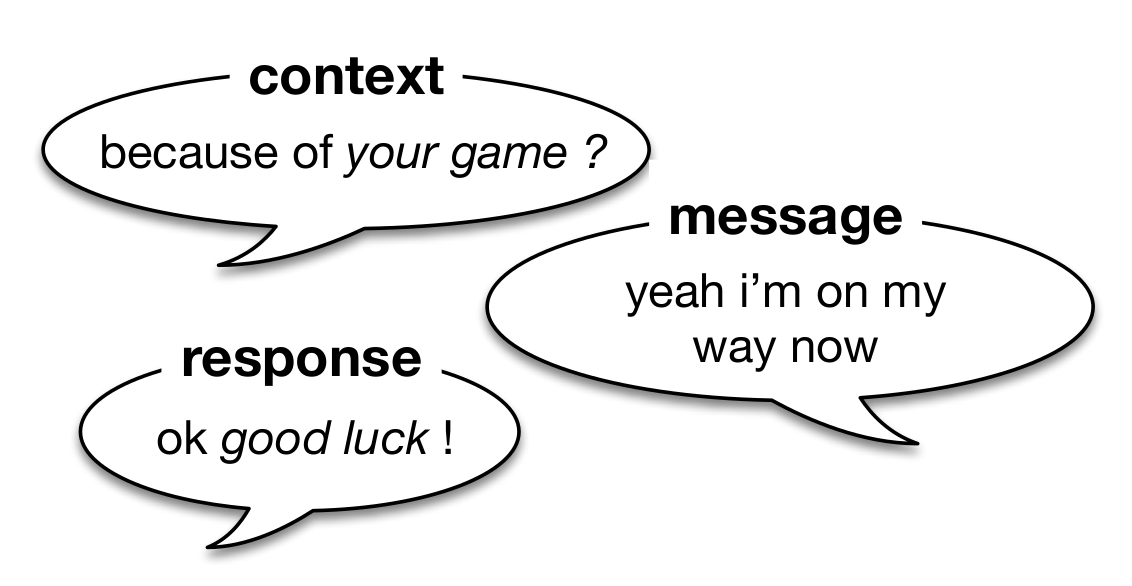
\includegraphics[width=0.6\textwidth]{figure/context_message_response.png}
    \centering
    \caption{上下文,消息和响应的关系\upcite{DCGM}}
    \label{fig:context_message_response}
\end{figure}

% -- Definitions -- %
下面定义面向闲聊的对话系统的主要术语。
本领域考察的场景是两个人交替的用文本(而不是语音)进行对话,
两人有先后顺序的各说一段话$x, y$,称为一轮对话$t = (x, y)$(Turn),
一个对话数据样本$D$是对话的序列$D = t_1, t_2, \dots, t_n$,
它至少包含一轮对话,
样本的最后一轮对话$t_n = (x_n, y_n)$称为当前轮,
序列$t_1, t_2, \dots, t_{n-1}$称为当前轮的上下文$c$,
$x_n$称为当前轮的消息$m$,$y_n$称为当前轮的响应$r$(在不引起歧义的情况下,“当前轮”可以省略)。
若样本只有一轮对话,则上下文为空序列。
$c,m,r$三者的关系如图~\ref{fig:context_message_response}~所示。
给定上下文$c$和消息$m$,模型需要预测响应$r$,
这就是对话响应生成问题(Dialogue Response Generation)。


% -- Generative System -- %
面向闲聊的对话系统又可以分为生成式系统(Generative System)和检索式系统(Retrieval System)
\upcite{corpus_survey,NUC},
两者的主要区别是产生输出的机制不同。
简单来说,如果一个系统能生成训练集里没有出现过的句子,
就把它称为生成式系统,反之则称为检索式系统\upcite{HowNot}。
生成式系统估计了给定输入特征$X$,预测结果为$Y$的条件概率$p(Y|X)$,
并输出使条件概率最大化的句子。
设$U$是所有句子的集合,生成式模型的输出机制可以表示为:
\begin{align}
    Y = \argmax_{Y'\in U} p(Y'|X)
\end{align}

% -- Retrieval System -- %
检索式系统根据输入特征$X$和数据集$C$中的候选输出$Y'$计算评分$\textit{Score}(X, Y')$,
并选出评分最高的候选。
为了使输出自然流畅而且不容易出现重复,$C$通常由大量人类撰写的语句组成。
常见的评分机制有
词频-逆文档频率(Term Frequency Inverse Document Frequency,TF-IDF)
和语义相似度(Semantic Similarity)等等。
检索式系统的输出机制可以表示为:
\begin{align}
    Y = \argmax_{Y'\in C} \textit{Score}(Y', X)
\end{align}

这两种方法各有优劣:检索式系统的输出没有语法错误并且可以对输出内容进行限制\upcite{NUC},但是不能生成新句子;
生成式系统可以生成新的句子\upcite{Shang},但是容易生成过短的句子\upcite{AdverEval}。
两种系统的联合体(Ensemble)通常能比单一系统获得更好的性能\upcite{Two_are_better_than_one}。
而在实验中,检索式系统也经常作为生成式系统的基线\upcite{Shang,DCGM}。

% -- Short Review of Technical Background -- %
生成式模型的流行得益于自然语言处理领域的一系列基础技术,包括
能为把单词转化为平滑的向量特征的词嵌入(Word Embedding)\upcite{NNLM,word2vec,Glove},
能更有效的对序列建模的循环神经网络语言模型(Recurrent Neural Networks Language Model,RNNLM)\upcite{RNNLM},
能避免梯度消失问题\upcite{VanishingGradient}的门单元,
如长短期记忆(Long Short-Term Memory,LSTM)\upcite{LSTM}和
带门循环单元(Gated Recurrent Unit,GRU)\upcite{GRU},
能端对端训练的序列到序列框架(Sequence to Sequence Framework,Seq2Seq)\upcite{Seq2Seq,GRU},
以及能改善长期依赖问题(Long-Span Dependency)的注意力机制\upcite{JointTransAlign,EffectiveAttention}。

% -- Chatbots Based on Seq2Seq -- %
这些技术促进了基于神经网络的机器翻译(Neural Machine Translation,NMT)的发展,
也促使学者们把机器翻译的技术应用到生成式对话上。
在国外,最早把Seq2Seq框架用到生成式对话的是Vinyals等人\upcite{GoogleChatbot},
他们在OpenSubtitles\upcite{opensub}
上训练的模型能回答简单的常识问题,
并且比基于规则的系统CleverBot\footnote{\url{http://www.cleverbot.com/}}获得了更高的人类评分。

% -- Li -- %
Li等人在增加响应的多样性方面做了一系列的工作。
他们提出把最大互信息作为解码的目标函数\upcite{MMI},
增加消息-响应和响应-消息两个方向的相关性。
他们提出的Persona模型\upcite{persona}在解码器端加入了说话人身份(Speaker ID),
有效的促进了响应的人格一致性(Personality Coherence)。
他们还把强化学习(Reinforcement Learning,RL)和
对抗生成网络(Generative Adversarial Networks,GAN)应用到响应生成问题上\upcite{deep_RL,Adversarial},
并取得了有意义的进展。

% -- Serban -- %
Serban等人扩展了Sordoni等人提出的多层编解码器\upcite{hred-qs},
并将其应用到对话生成领域\upcite{HRED}。
基于多层编解码器,Serban等人又提出了利用随机隐变量增加对话多样性的隐变量多层编解码器\upcite{VHRED},
以及加入了高层次抽象信息的多精度循环神经网络(Multiresolution Recurrent Neural Networks,MrRNN)\upcite{MrRNN}。

% -- Shang -- %
在国内,Shang等人研究了基于新浪微博数据集的短文本对话生成问题\upcite{Shang},
并提出了以GRU为门单元的编解码器模型(Neural Response Machine,NRM)。
他们的模型在人类评价上取得了比检索式系统和基于统计机器翻译
(Statistical Machine Translation,SMT)的系统更好的成绩。
Xing等人提出了能利用主题词的Seq2Seq模型\upcite{Topic_Aware},
由于篇幅有限,不能一一介绍。


\section{课题研究意义}\label{sec:research_meaning}
本领域目前面临两个难题:
一是如何合理评价生成式系统的性能\upcite{HowNot,Shang,deep_RL,deltaBLEU,ADEM},
二是如何避免生成单调无意义的响应,增加响应的多样性\upcite{MMI,Distill,Ritter11,DCGM,HRED},
本课题致力于解决第一个难题。
如表~\ref{tab:multiple_valid_responses}~所示,
对于一则给定的消息,合理响应的数量不止一个。
虽然在机器翻译领域,对于源句子的合理翻译也可以有多个,
但是这些翻译必须在语义上和参考大体一致,并且和源句子的语义完全相同,
所以,机器翻译的合理输出之间只存在语法和词法层面的多样性。
而在对话响应生成领域,尽管什么是合理的响应还没有一个明确的定义,
但从直观上来看,对一个消息的回答不应该是该消息的语义重复,
所以合理的响应不需要和消息保持语义一致性。
对合理响应更少的约束条件意味着更大的可能性空间。
这种固有的多样性导致评价响应生成系统比评价机器翻译系统困难。
\begin{table}
    \centering
    \caption{合理的响应不唯一\upcite{RUBER}}
    \label{tab:multiple_valid_responses}
    \begin{tabular}{rl}
        \toprule
        \midrule
        \textbf{消息:} & 为什么不领养一个? \\
        & Why not adopt one? \\
        \textbf{参考:} & 我也想领养,但是不好找。 \\
        & I hope so, but it's hard to find one. \\
        \midrule
        \textbf{响应1:} & 恩,我已经在朋友中找了。 \\
        & I'm looking for one from my friends. \\
        \textbf{响应2:} & 巴比伦是稀有品种。 \\
        & Pappilon is a rare breed. \\
        \textbf{响应3:} & 可以哈。谢谢你的建议。 \\
        & OK, thank you for your advice. \\
        \bottomrule
    \end{tabular}
\end{table}

本文试图通过实验证实评价生成式模型的困难性,并指出导致这种困难性的几个方面的原因。
虽然,目前大多数评价指标尚不具有和人类评价较高的一致性,
但是对它们的研究将有助于理解现有指标的弱点,从而有助于自动化评估的发展。
尽管没有使用人类评价,本文对评价指标、模型和数据集的分析还是取得了有意义的结论。

\section{课题研究内容}\label{sec:reseach_content}
Liu等人发现自动评价指标在非技术性的Twitter对话数据集上和人类评价只有弱相关性,
在技术性的Ubuntu对话数据集上和人类评价没有相关性\upcite{HowNot}。
本文延续Liu等人的工作,
研究了评价指标之间的相关性,以及模型的性能在不同数据集上的迁移能力。

本文以Serban等人在文献\cite{VHRED}的实验中使用的三个模型LSTM,HRED,VHRED为基线,
扩展了Liu等人在文献\cite{HowNot}中考察的两类指标,即基于词重叠的指标和基于词嵌入的指标,
在三个具有代表性的公开数据集,Ubuntu对话数据集,OpenSubtitles和LSDSCC上进行了实验。

\section{论文组织结构}\label{sec:paper_organization}
本文的组织结构如下:
第~\ref{ch:related_work}~章相关工作介绍了生成式模型的基本定义以及指标和数据集的基本情况。
第~\ref{ch:method}~章研究方法介绍了本文的实验框架,模型超参数,数据集预处理和指标参数的选择等等。
第~\ref{ch:experiment}~章实验结果与讨论详细展示了实验数据和结论。
最后一章结论总结了本文的研究成果,提出了若干研究方向。
